%%%% main.tex --- IJCAI-ECAI 2026 CFD Workshop submission
%%%% Carry-Over Lottery Allocation: family + manipulation bound

\typeout{IJCAI-ECAI 26 CFD Workshop submission}

\documentclass{article}
\pdfpagewidth=8.5in
\pdfpageheight=11in

\usepackage{ijcai26}

\usepackage{times}
\usepackage{soul}
\usepackage{url}
\usepackage[hidelinks]{hyperref}
\usepackage[utf8]{inputenc}
\usepackage[small]{caption}
\usepackage{graphicx}
\usepackage{amsmath}
\usepackage{amssymb}
\usepackage{amsthm}
\usepackage{booktabs}
\usepackage{multirow}
\usepackage{algorithm}
\usepackage{algorithmic}
\usepackage[switch]{lineno}
\usepackage{natbib}

% Line numbers required for submission per IJCAI guidelines.
% Comment out for camera-ready.
\linenumbers

\urlstyle{same}

% Theorem environments
\newtheorem{theorem}{Theorem}
\newtheorem{lemma}[theorem]{Lemma}
\newtheorem{proposition}[theorem]{Proposition}
\newtheorem{corollary}[theorem]{Corollary}
\newtheorem{definition}{Definition}
\newtheorem{remark}{Remark}

% Macros
\newcommand{\cola}{\textup{\textsc{Cola}}}
\newcommand{\Max}{\textup{\textsc{Max}}}
\newcommand{\E}{\mathbb{E}}
\newcommand{\Prob}{\mathbb{P}}

% Required PDF info per IJCAI template (pdftex primitive).
% Guard against engines without \pdfinfo (e.g., XeTeX-based tectonic)
% so the document still compiles for local preview. Reviewers will use
% pdftex / pdflatex which honors this primitive.
\makeatletter
\@ifundefined{pdfinfo}{\def\pdfinfo#1{}}{}
\makeatother
\pdfinfo{
/TemplateVersion (IJCAI.2026.0)
}

\title{An Analytic Manipulation Bound for the Carry-Over Lottery Allocation Family}

\author{
Timothy Highley$^1$
\and
Kaushik Rajan$^2$
\\
\affiliations
$^1$La Salle University \\
$^2$Independent researcher \\
\emails
highley@lasalle.edu, kaushi@alumni.ncsu.edu
}

\begin{document}

\maketitle

\begin{abstract}
The National Basketball Association (NBA) draft lottery is a fair-allocation problem with a documented manipulation incentive: teams eliminated from playoff contention can improve their expected draft position by losing additional games. \citet{munro2020notanking} prove an impossibility result: no mechanism mapping end-of-season records to draft probabilities can simultaneously reward poor performance and eliminate this incentive. Carry-Over Lottery Allocation (\cola{}) sidesteps the impossibility by replacing single-season records with multi-year playoff history as the basis for draft priority \citep{highley2026cola}. The mechanism's incentive-compatibility argument relies on five assumptions, four of which hold by construction; the fifth---that pool-manipulation gains are negligible---is supported by simulation but lacks a closed-form bound. We make two contributions. First, we derive an analytic upper bound of approximately 4\% on the worst-case probability gain from pool manipulation under empirically calibrated index distributions, with a closed-form sensitivity to the underlying parameters. Second, we present a brief historical backtest (26 NBA seasons, five variants) and an analytic per-series bound for Capped \cola{}, the variant introduced in response to recent NBA reform discussions. We also surface an open mapping between the \cola{} family and the axiomatic draft-rule literature \citep{coreno2022axiomatic}.
\end{abstract}

\section{Introduction}

The annual NBA draft allocates a small number of indivisible items (draft picks) to a fixed set of agents (the league's 30 teams). Among the 30 teams, the 14 that miss the playoffs participate in a lottery for the top picks; the rest receive picks in reverse order of regular-season record. The lottery is the focus of our paper because it carries the policy weight: it determines who gets the franchise-altering top picks each year, and its design has been revised three times in 60 years to address an empirically observed manipulation incentive known as \emph{tanking}. A team eliminated from playoff contention can improve its expected draft position by losing additional games, and the design of any priority rule must contend with this.

\citet{munro2020notanking} formalise the tension as an impossibility. They define a \emph{No-Tanking Condition} (NTC): no team can improve its expected outcome by losing. Under NTC and the requirement that worse-record teams receive strictly better draft odds, only a uniform lottery (equal odds for all non-playoff teams) survives---abandoning the goal of helping the weakest teams. The 2026 NBA reform proposal known as ``3-2-1'' takes precisely this route, with adjustments for play-in-tournament eligibility \citep{highley2026solvable5}.

Carry-Over Lottery Allocation (\cola{}) sidesteps the impossibility by replacing single-season records with multi-year playoff history as the basis for draft priority \citep{highley2026cola}. Each non-playoff team accumulates lottery tickets over consecutive seasons of missed playoffs; success in the playoffs or in the draft itself diminishes a team's accumulated tickets. The single-season manipulation channel that drives the Munro-Banchio counterexample becomes ineffective because no single-season choice materially shifts the multi-year ticket pool.

\paragraph{Our contributions.}
\begin{itemize}
    \item \textbf{An analytic manipulation bound.} \cola{}'s incentive-compatibility argument rests on five assumptions, four of which hold by construction. The fifth---pool manipulation gains are negligible---is supported in the original paper by simulation over 1{,}000 synthetic seasons. We derive a closed-form upper bound of approximately 4\% on the worst-case probability gain, with explicit sensitivity to the underlying index-distribution parameters (Section~\ref{sec:bound}). The bound contains the simulation-observed extremes and provides the first parameter-explicit ceiling.
    \item \textbf{A family-level perspective.} We present the \cola{} mechanism family (Section~\ref{sec:family}) as five variants on a shared scaffold, including \emph{Capped \cola{}}, the variant introduced in response to NBA-side feedback to bound the per-series cost of advancing in the playoffs. We derive an analytic per-series bound for Capped \cola{} (Lemma~\ref{lem:capped-bound}). Empirical results from a 26-season historical backtest (Section~\ref{sec:empirical}) calibrate the bounds.
    \item \textbf{A bridge to the axiomatic fair-division literature.} \citet{coreno2022axiomatic} establish an impossibility for draft rules satisfying Respect for Priority, Envy-Free up to One Object, and Strategy-Proofness simultaneously. We surface a preliminary mapping between \cola{}'s priority structure and these axioms (Section~\ref{sec:fairdiv}) as an invitation for further axiomatic analysis.
\end{itemize}

\section{Background and Related Work}
\label{sec:background}

\subsection{Effort Manipulation: The Munro-Banchio Impossibility}

\citet{munro2020notanking} establish that any mechanism mapping end-of-season records to draft probabilities, while giving worse teams strictly better odds, must violate NTC. The proof constructs a minimal counterexample: two teams, both eliminated, with identical records and a final game against each other. The loser finishes with a worse record and therefore receives better draft odds; both teams prefer to lose. Only the uniform lottery satisfies NTC, but uniform odds abandon the goal of differential reward.

The authors propose an alternative, \emph{T-IC} (Truncated Incentive Compatibility), which tracks each team's conditional probability of finishing last and freezes allocations at the moment IC would first be violated. T-IC is optimal in theory but computationally expensive, opaque to fans, and limited to single-season scope; calculation requires precise team-level valuations of playoff-versus-draft trade-offs that the league does not have, and some teams have an incentive to tank from the first game of the season, which the truncation timing does not reach.

\subsection{Preference Manipulation: The Coreno-Balbuzanov Impossibility}
\label{sec:fairdiv}

\citet{coreno2022axiomatic} address a complementary manipulation vector: teams misreporting which players they prefer. They prove that no allocation rule simultaneously satisfies:
\begin{itemize}
    \item \textbf{Respect for Priority (RP):} higher-priority teams receive weakly better allocations~\citep{svensson1994allocation};
    \item \textbf{Envy-Free up to One Object (EF1):} no team envies another's allocation after removing one item~\citep{lipton2004approximately,budish2011combinatorial};
    \item \textbf{Strategy-Proofness (SP):} no team benefits from misreporting preferences.
\end{itemize}

The constituent axioms trace to peer-reviewed sources. RP extends Svensson's ``weak fairness'' from queue allocation to draft priority \citep{svensson1994allocation}. EF1 originates with \citep{lipton2004approximately} and is adapted to the indivisible-goods assignment setting by \citep{budish2011combinatorial}.

Whether RP and EF1 lift from single-period draft rules to \cola{}'s multi-year mechanism is an open question. A preliminary reading: under \cola{}, longer droughts produce weakly better expected draft position, which mirrors RP if priority is identified with the multi-year ticket ranking; the graduated diminishment schedule preserves EF1 in the sense that no team prefers another's outcome once one ``lucky'' lottery win is removed. We do not assert this lift; we surface it as an axiomatic question that the workshop's audience is well placed to resolve.

\section{The COLA Mechanism Family}
\label{sec:family}

\subsection{Common Framework}

Every \cola{} variant maintains a per-team, integer-valued state across seasons and uses that state to determine draft priority in the current season. We refer to this state as the \emph{lottery index} and write $L_i^{(t)}$ for team $i$ at the end of season $t$.

\begin{definition}[Lottery Index]
\label{def:index}
For each team $i$ and season $t$, the lottery index $L_i^{(t)} \in \mathbb{Z}_{\geq 0}$ is determined by an initial value $L_i^{(0)}$, a per-season \emph{increment} $\Delta_i^{(t)}$ (variant-specific), and a per-season \emph{diminishment} $\rho_i^{(t)} \in [0, 1]$ that scales the index down based on playoff and draft outcomes:
\begin{equation*}
L_i^{(t+1)} = \left(L_i^{(t)} + \Delta_i^{(t)}\right) \cdot \left(1 - \rho_i^{(t)}\right).
\end{equation*}
The \emph{pool} in season $t$ is $P^{(t)} = \sum_{i \in E^{(t)}} L_i^{(t)}$, where $E^{(t)}$ is the set of teams eligible for the lottery.
\end{definition}

The three components --- the eligibility set $E^{(t)}$, the increment $\Delta_i^{(t)}$, and the diminishment $\rho_i^{(t)}$ --- are the levers that distinguish the variants.

\subsection{Five Variants}

\paragraph{Simple \cola{}} eliminates the lottery: eligibility is the 22 teams with zero playoff series wins (14 non-playoff teams + 8 first-round losers). Teams are ranked by drought (consecutive seasons without a playoff series win or top-3 lottery pick), tiebroken by most regular-season wins. Picks are assigned deterministically.

\paragraph{Simple Lottery \cola{}} shares Simple's drought state and 22-team pool. Pre-2019 NBA lottery odds (25.0\% down to 0.5\% across the worst 14 teams) are applied to the top 14 by drought; the remaining 8 receive picks 15--22 deterministically.

\paragraph{Classic \cola{}} is the variant developed in detail by \citet{highley2026cola} and the variant our manipulation bound directly analyses. The eligibility set is the 14 non-playoff teams; each non-playoff team receives an increment of $\alpha = 1{,}000$ tickets per season; playoff teams receive zero increment. Diminishment is graduated: champion ($\rho = 1.0$), finals ($0.75$), conference finals ($0.5$), second round ($0.25$), first round ($0$); draft pick \#1 ($\rho = 1.0$), \#2 ($0.75$), \#3 ($0.5$), \#4 ($0.25$), \#5 and below ($0$). The lottery for picks 1--4 is weighted by lottery index ($p_i = L_i / P$); picks 5--14 are assigned by lottery-index rank.

\paragraph{Countdown \cola{}} ranks teams by McCarty number $M_i = d_i \cdot w_i$ (drought $\times$ regular-season wins). The same 22-team pool as Simple \cola{} is partitioned into nested 5-team \emph{elimination pools}; draft picks are assigned bottom-up via ticket allocation $(2, 3, 4, 5, 6)$ within each pool. The mechanism guarantees that no team falls more than four spots below its rank.

\paragraph{Capped \cola{}} \citep{highley2026solvable5} caps the lottery index at $\Max$ (default 150). The increment is $\Delta_i^{(t)} = w_i^{(t)}$ for any team finishing the regular season outside the top 6 of either conference; eligibility excludes (i) teams that won a top-5 lottery pick last season and (ii) teams that won a playoff series this season or last. Diminishment uses a six-step playoff schedule (champion, runner-up, conference finals, second round, first round, play-in winner losing R1) and a five-step draft schedule, smoothing the cliffs of Classic \cola{}.

\subsection{Incentive Compatibility}

\citet{highley2026cola} establish IC for Classic \cola{} under five assumptions:
\begin{enumerate}
    \item \textbf{Playoff primacy:} the value to a team of advancing in the playoffs exceeds the value of any plausible draft-pick gain.
    \item \textbf{Playoff advancement:} within the playoffs, advancing further is preferred to losing earlier, controlling for opponent strength.
    \item \textbf{Picks 5--14 negligible at the margin:} no team profits from manipulating its position among those slots through within-season effort.
    \item \textbf{Pool manipulation negligible:} no team can meaningfully shift its expected draft position by manipulating which other teams are in or out of the lottery pool.
    \item \textbf{No traded-pick protections:} pick trades do not interact with diminishment in a way that creates manipulation incentives.
\end{enumerate}
Assumptions (1)--(3) and (5) hold by construction or follow from straightforward arguments. Assumption (4) is the open one: \citet{highley2026cola} support it via 1{,}000-season simulation, observing a maximum probability gain of approximately 3\%. The next section converts this empirical observation into a closed-form analytic bound.

\section{Pool Manipulation Bound}
\label{sec:bound}

\subsection{Setup}

Let $P = \sum_{i=1}^{n} L_i$ denote the total lottery pool, where $L_i$ is team $i$'s lottery index and $n$ is the number of lottery-eligible teams. A team's probability of winning the first pick is $p_i = L_i / P$.

The \emph{pool manipulation} channel operates as follows. Team $i$ deliberately loses to a high-index opponent $h$ near the playoff boundary, causing $h$ to make the playoffs. Team $h$ (with index $L_h$) exits the lottery pool and is replaced by a lower-index team $\ell$ (with index $L_\ell < L_h$). The pool shrinks by $\Delta = L_h - L_\ell > 0$.

\begin{proposition}[Manipulation Gain]
\label{prop:gain}
The probability gain for team $i$ from a pool swap of size $\Delta = L_h - L_\ell$ is
$
G_i = \frac{L_i \cdot \Delta}{P \cdot (P - \Delta)}.
$
\end{proposition}

\begin{proof}
Before manipulation, $p_i = L_i / P$. After the swap, the new pool is $P' = P - \Delta$ and $p_i' = L_i / P'$. The gain is $G_i = p_i' - p_i = L_i \left(\frac{1}{P - \Delta} - \frac{1}{P}\right) = \frac{L_i \cdot \Delta}{P(P - \Delta)}$.
\end{proof}

When $\Delta \ll P$, the gain factors into two ratios: the manipulator's pool share ($p_i$) and the fractional pool change ($\Delta / P$). Both have structural ceilings.

\subsection{Conditioned Upper Bound}

\begin{definition}[Structural Anti-Correlation]
\label{def:anticorr}
Let $T_{\max}$ denote the maximum consecutive non-playoff years for any team, and $T_{\text{boundary}}$ the maximum consecutive non-playoff years for a team near the playoff boundary (i.e., a team that could plausibly be pushed into the playoffs by a single loss). The index distribution exhibits \emph{structural anti-correlation} when $T_{\text{boundary}} \ll T_{\max}$: teams with the highest indices are far from the playoff boundary and thus cannot be the target of pool manipulation.
\end{definition}

\begin{theorem}[Conditioned Manipulation Bound]
\label{thm:bound}
Under structural anti-correlation with parameters $T_{\max}$, $T_{\text{boundary}}$, and average index multiplier $\bar{k} = \bar{L} / \alpha$, the maximum manipulation gain satisfies
\begin{equation*}
G_{\max} \leq \frac{T_{\max} \cdot (T_{\text{boundary}} - 1)}{(T_{\max} + n - 1) \cdot n \cdot \bar{k}}.
\end{equation*}
\end{theorem}

\begin{proof}[Proof sketch]
The gain is maximised when $L_i$ is maximised and $\Delta / P$ is maximised. \textbf{Bounding $p_{\max}$:} the highest-index team has $L_{\max} = T_{\max} \cdot \alpha$. The minimum pool size occurs when one team has $T_{\max}$ years of accumulation and the remaining $n-1$ teams each have the minimum $\alpha$: $P_{\min} = (T_{\max} + n - 1) \cdot \alpha$. Thus $p_{\max} \leq T_{\max} / (T_{\max} + n - 1)$. \textbf{Bounding $\Delta / P$:} the team being pushed out has at most $T_{\text{boundary}} \cdot \alpha$ tickets, and the team replacing it has at least $\alpha$, so $\Delta_{\max} = (T_{\text{boundary}} - 1) \cdot \alpha$. In steady state, $P \approx n \cdot \bar{k} \cdot \alpha$. Combining via the first-order approximation yields the stated bound.
\end{proof}

\paragraph{Empirical calibration.} Using $T_{\max} = 10$ (the longest observed steady-state non-playoff stretch in our 26-season backtest), $T_{\text{boundary}} = 5$, $n = 14$, and $\bar{k} = 3.1$ (an average team has roughly three years of carry-over before reset, matching the original paper's observation), we obtain
$
G_{\max} \leq 10 \cdot 4 / (23 \cdot 14 \cdot 3.1) \approx 4.0\%.
$
This contains the simulation-observed maximum of 3.0\% across 1{,}000 seasons \citep{highley2026cola} with approximately $1.3\times$ headroom. An independent 200-season Bradley-Terry simulation we ran confirms the bound, with observed maximum gain of 1.70\% (Figure~\ref{fig:bound}).

\begin{figure}[t]
\centering
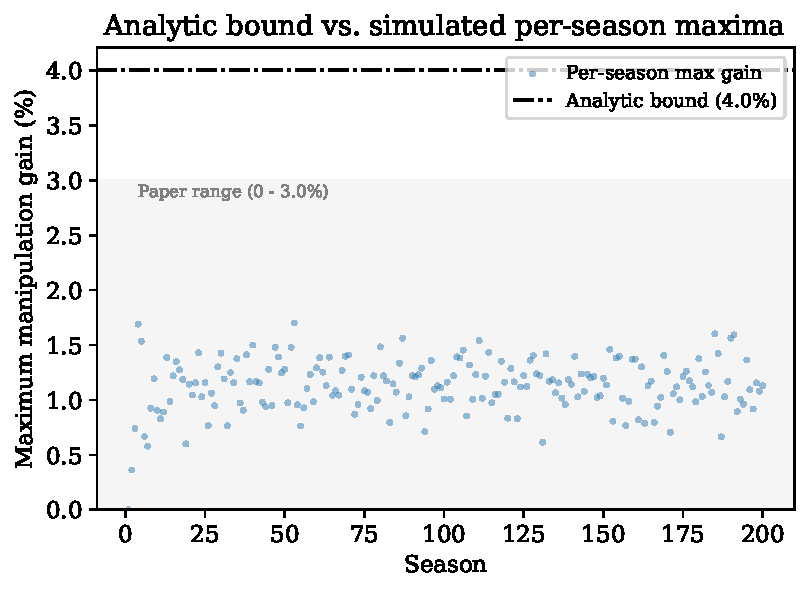
\includegraphics[width=\columnwidth]{figures/bound_vs_sim.pdf}
\caption{Analytic bound (red) vs.\ simulation distribution across 200 Bradley-Terry seasons. The bound contains all simulated outcomes with margin.}
\label{fig:bound}
\end{figure}

\subsection{Per-Series Bound for Capped \cola{}}

Capped \cola{} introduces a fourth manipulation channel: tanking through the playoffs themselves (declining to advance in order to retain stockpile). The cap converts the playoff-diminishment schedule from a fraction-of-current-stockpile cost (unbounded above when the stockpile grows large) to a fraction-of-$\Max$ cost (bounded by construction).

\begin{lemma}[Per-Series Tanking Cost]
\label{lem:capped-bound}
Let $\Max$ be the Capped \cola{} stockpile cap. For any team entering the playoffs with $L_i \leq \Max$, the maximum reduction in $L_i$ attributable to winning (rather than losing) any single playoff series is bounded by:
\begin{equation*}
\Delta L_{\text{series}}^{\max} = \begin{cases}
0.3 \cdot \Max & \text{play-in advancers in round 1,} \\
0.2 \cdot \Max & \text{any other series advancement.}
\end{cases}
\end{equation*}
At $\Max = 150$, the bound is 45 tickets for the play-in case and 30 tickets for each subsequent series.
\end{lemma}

\begin{proof}
Reading off Capped \cola{}'s six-step diminishment schedule, the per-series increments in the diminishment fraction $\Delta\rho$ are: play-in advancer round 1 ($\rho_{\text{lose}} = 0.1$, $\rho_{\text{advance}} = 0.4$, $\Delta\rho = 0.3$); standard round 1 ($0.2 \to 0.4$, $\Delta\rho = 0.2$); round 2 ($0.4 \to 0.6$); conference finals ($0.6 \to 0.8$); finals ($0.8 \to 1.0$). All non-play-in transitions yield $\Delta\rho = 0.2$. The cost in tickets is $\Delta\rho \cdot L_i^{\text{pre}} \leq \Delta\rho \cdot \Max$, with equality at the cap.
\end{proof}

The bound makes the playoff-tanking incentive transparent at the league level: at $\Max = 150$, no single series win ever costs a team more than 45 lottery tickets, which is approximately a year and a half of accumulation for a team near the wins-increment ceiling.

\section{Empirical Validation}
\label{sec:empirical}

\subsection{Backtesting Engine}

We compute \cola{} state for every team across 26 NBA seasons (1999--2025), using verified Basketball Reference data: 775 team-season records, 776 first-round draft picks, and 55 lottery-day-attributed pre-draft pick trades. The engine separates pre-draft state (Phase A, used for draft probability calculations) from post-draft diminishment (Phase B, carried forward to the next season). Cold-start effects stabilise by approximately season 5; we report aggregates over the 21 stable seasons (2005--2025).

\subsection{Capped COLA Cap Calibration}

Capped \cola{} is parameterised by a single tunable constant $\Max$. The cap controls the trade-off between (i) ordering resolution at the top of the lottery (a higher cap permits more separation between the highest-stockpile teams) and (ii) the per-series tanking exposure of Lemma~\ref{lem:capped-bound} (a higher cap raises the maximum cost of advancing past round 1). Table~\ref{tab:cap-sweep} reports the 21-stable-season aggregates from a sweep over $\Max \in \{75, 100, 125, 150, 175, 200\}$.

\begin{table*}[t]
\centering
\small
\begin{tabular}{rccccc}
\toprule
$\Max$ & Teams at cap (mean) & Teams at cap (max) & Sep.\ R1--R5 (mean) & Per-series cost (max) & Cum.\ regret (max) \\
\midrule
75  & 6.71 & 9 &  0.9 & 22.5 & 45.0 \\
100 & 4.33 & 8 & 11.7 & 30.0 & 53.7 \\
125 & 2.86 & 4 & 27.9 & 37.5 & 53.7 \\
\textbf{150} & \textbf{1.62} & \textbf{3} & \textbf{47.7} & \textbf{45.0} & \textbf{57.6} \\
175 & 0.95 & 2 & 65.4 & 52.5 & 67.2 \\
200 & 0.52 & 2 & 76.4 & 60.0 & 76.8 \\
\bottomrule
\end{tabular}
\caption{Capped \cola{} aggregates across 21 stable seasons (2005--2025). Per-series cost max $= 0.3 \cdot \Max$ from Lemma~\ref{lem:capped-bound}; cumulative regret max is the worst empirical observation. The bolded $\Max = 150$ row is the variant's published default \citep{highley2026solvable5}.}
\label{tab:cap-sweep}
\end{table*}

Three patterns emerge. Sub-100 caps over-compress the lottery: at $\Max = 75$, more than six teams sit at the cap on average and the rank-1 vs.\ rank-5 separation collapses to under 1 ticket. Caps above 175 erase the cap's purpose: fewer than one team sits at the cap on average. The published $\Max = 150$ choice produces fewer than two teams at the cap in 19 of 21 stable seasons and at most three in any single season, matching the variant's published headline ``no more than three teams at the maximum at a time, and on average fewer than two.''

\subsection{Cross-Variant Comparison}

The five variants rank teams differently under identical historical data. In 2024--25, the Sacramento Kings lead Classic \cola{}'s ticket pool (16-season drought, accumulated index 11{,}250) but Chicago leads Simple, Simple Lottery, and Countdown \cola{} (longest-running multi-year stretch by drought count alone). Capped \cola{} places multiple teams at the cap simultaneously, eliminating the differential between long-rebuilding franchises in a single year and trading resolution for a bounded per-series exposure.

\section{Discussion}
\label{sec:discussion}

The bounds in this paper establish that \cola{}'s open assumption (4) is bounded by approximately 4\% under empirically calibrated parameters, and that the additional manipulation channel introduced by Capped \cola{}'s cap is bounded at $0.3 \cdot \Max$ tickets per series. Combined, the four manipulation channels available under Capped \cola{}---single-season tanking (zero, by construction), pool manipulation ($\sim$4\% probability gain), multi-year strategic tanking (bounded by the diminishment schedule), and per-series playoff tanking (45 tickets at $\Max = 150$)---compose to a small joint exposure relative to the status-quo lottery, where repeat tanking has memoryless returns.

The 2026 NBA reform proposal known as ``3-2-1'' adopts a different escape from the Munro-Banchio impossibility: it expands the lottery to 16 teams with a bounded-spread ball allocation that approximates the uniform lottery within an adjustment for the play-in tournament. The proposal includes a three-year re-evaluation provision \citep{highley2026solvable5}. \cola{}'s contribution to that re-evaluation conversation is the multi-year-history dimension that 3-2-1 omits, and the bounds in this paper formalise the manipulation properties that any future-iteration discussion will need.

Two open directions extend this work. First, the structural anti-correlation in Definition~\ref{def:anticorr} is calibrated, not formally derived; a stationarity argument that bounds $T_{\text{boundary}}$ as a function of league parameters would close Assumption (4) entirely. Second, the lift from \citet{coreno2022axiomatic}'s axioms to multi-period priority mechanisms (Section~\ref{sec:fairdiv}) is open: whether \cola{}'s ticket ordering satisfies RP and EF1 in a formal sense is a fair-division question on which workshop participants are well placed to make progress.

\bibliographystyle{named}
\bibliography{references}

\end{document}
